\documentclass[12pt,a4paper]{article}

\usepackage[margin=1in]{geometry}
\usepackage{graphicx}
\usepackage{booktabs}
\usepackage{amsmath}
\usepackage{float}
\usepackage{hyperref}
\usepackage{array}
\usepackage{setspace}

\onehalfspacing

\title{Stock Market Risk and Return Analysis}
\author{Nathan}
\date{\today}

\begin{document}

\maketitle

\begin{abstract}
This report analyses historical daily market data for Apple, Microsoft, NVIDIA, Amazon, the S\&P 500, and the FTSE 100 from 4 January 2010 to 31 December 2025. The aim is to understand how return, volatility, drawdown, and correlation differ across individual technology stocks and wider market indices. The analysis finds that NVIDIA produced the highest total return, but also had the highest volatility and the largest maximum drawdown. The results support the idea that higher long-term return is often linked with higher risk, although the relationship is not perfect. Microsoft, for example, produced a lower total return than Apple and Amazon, but had a strong risk-adjusted return based on the Sharpe ratio.
\end{abstract}

\section{Introduction}

Stock market investing involves a trade-off between risk and return. Investors usually want higher returns, but higher returns often come with greater uncertainty, larger price swings, and deeper temporary losses. This project investigates that relationship using real historical price data.

The purpose of this report is not to create a short-term trading system or claim that stock prices can be predicted perfectly. Instead, the aim is to use data analysis to answer clear financial questions:

\begin{itemize}
    \item Which assets grew the most over the study period?
    \item Which assets were the most volatile?
    \item Which assets experienced the largest drawdowns?
    \item Which assets tended to move together?
    \item Was higher return linked to higher risk?
\end{itemize}

The report focuses on exploratory data analysis, visualisation, and interpretation of key financial metrics.

\section{Data}

The dataset contains daily market data downloaded from Yahoo Finance. The assets included in the analysis are shown in Table \ref{tab:assets}.

\begin{table}[H]
\centering
\begin{tabular}{ll}
\toprule
Asset & Description \\
\midrule
Apple & Large US technology company \\
Microsoft & Large US technology company \\
NVIDIA & US semiconductor and artificial intelligence company \\
Amazon & US e-commerce and cloud computing company \\
S\&P 500 & Broad US stock market index \\
FTSE 100 & Broad UK stock market index \\
\bottomrule
\end{tabular}
\caption{Assets included in the analysis.}
\label{tab:assets}
\end{table}

The main study period runs from 4 January 2010 to 31 December 2025. The cleaned dataset contains daily closing prices, opening prices, high prices, low prices, and trading volume where available. The analysis mainly uses closing prices because closing prices are commonly used to calculate daily returns and long-term performance.

\section{Methodology}

\subsection{Daily Return}

Daily return measures the percentage change in an asset's closing price from one trading day to the next. It is calculated as:

\begin{equation}
    r_t = \frac{P_t - P_{t-1}}{P_{t-1}}
\end{equation}

where \(P_t\) is the closing price on day \(t\), and \(P_{t-1}\) is the closing price on the previous trading day.

Daily returns are useful because they allow assets with very different price levels to be compared fairly. For example, a \pounds 5 move in one stock is not the same as a \pounds 5 move in another stock if their starting prices are different. Percentage returns solve this problem.

\subsection{Total Return}

Total return measures how much an asset grew across the full period:

\begin{equation}
    \text{Total Return} = \frac{P_{\text{final}}}{P_{\text{initial}}} - 1
\end{equation}

This metric gives a clear view of long-term growth. However, it does not explain how risky or unstable the journey was.

\subsection{Annualized Return}

Annualized return converts the total return into an average yearly growth rate. This makes it easier to compare assets over long periods:

\begin{equation}
    \text{Annualized Return} = (1 + \text{Total Return})^{252/n} - 1
\end{equation}

where \(n\) is the number of daily return observations and 252 is used because there are approximately 252 trading days in a year.

\subsection{Volatility}

Volatility measures how much daily returns move around their average. In this report, volatility is calculated as the standard deviation of daily returns, annualized using:

\begin{equation}
    \text{Annualized Volatility} = \sigma_{\text{daily}} \times \sqrt{252}
\end{equation}

A higher volatility means the asset had larger daily price movements. This is interpreted as higher risk because the investment value was less stable.

\subsection{Sharpe Ratio}

The Sharpe ratio measures return relative to volatility:

\begin{equation}
    \text{Sharpe Ratio} = \frac{\text{Annualized Return}}{\text{Annualized Volatility}}
\end{equation}

This project uses a simplified Sharpe ratio with a zero risk-free rate. A higher Sharpe ratio means an asset produced more return for each unit of volatility. This helps compare assets that may have different levels of risk.

\subsection{Maximum Drawdown}

Maximum drawdown measures the largest fall from a previous peak to a later low:

\begin{equation}
    \text{Drawdown}_t = \frac{P_t}{\max(P_1, P_2, ..., P_t)} - 1
\end{equation}

The maximum drawdown is the worst value of this series. It is important because investors do not only care about final returns; they also care about how painful the largest temporary loss would have been.

\subsection{Correlation}

Correlation measures how similarly two assets move based on their daily returns. A correlation close to 1 means two assets often move in the same direction. A correlation close to 0 means there is no strong linear relationship. A negative correlation means two assets often move in opposite directions.

\section{Results}

\subsection{Summary Metrics}

Table \ref{tab:summary} summarises the main risk and return metrics.

\begin{table}[H]
\centering
\small
\begin{tabular}{lrrrrr}
\toprule
Asset & Total Return & Annual Return & Volatility & Sharpe & Max Drawdown \\
\midrule
NVIDIA & 43,906\% & 46.4\% & 45.7\% & 1.02 & -66.3\% \\
Apple & 4,136\% & 26.4\% & 28.2\% & 0.94 & -43.8\% \\
Amazon & 3,348\% & 24.8\% & 32.8\% & 0.76 & -56.1\% \\
Microsoft & 1,991\% & 21.0\% & 25.5\% & 0.82 & -37.1\% \\
S\&P 500 & 504\% & 11.9\% & 17.3\% & 0.69 & -33.9\% \\
FTSE 100 & 81\% & 3.8\% & 15.5\% & 0.24 & -36.6\% \\
\bottomrule
\end{tabular}
\caption{Risk and return summary from 2010 to 2025.}
\label{tab:summary}
\end{table}

NVIDIA had the highest total return by a very large margin. Its total return of approximately 43,906\% means the final closing price was around 440 times higher than the starting closing price. Apple and Amazon also produced very strong returns, but they were far below NVIDIA.

The broad market indices had much lower total returns. The S\&P 500 returned approximately 504\%, while the FTSE 100 returned approximately 81\%. This difference shows how strongly the selected US technology stocks outperformed the two wider market benchmarks during this period.

\section{Visual Analysis}

\subsection{Growth of One Unit Invested}

Figure \ref{fig:growth} shows the growth of one unit invested in each asset at the start of the period. This chart normalises all assets to the same starting value, which makes their growth paths easier to compare.

\begin{figure}[H]
\centering
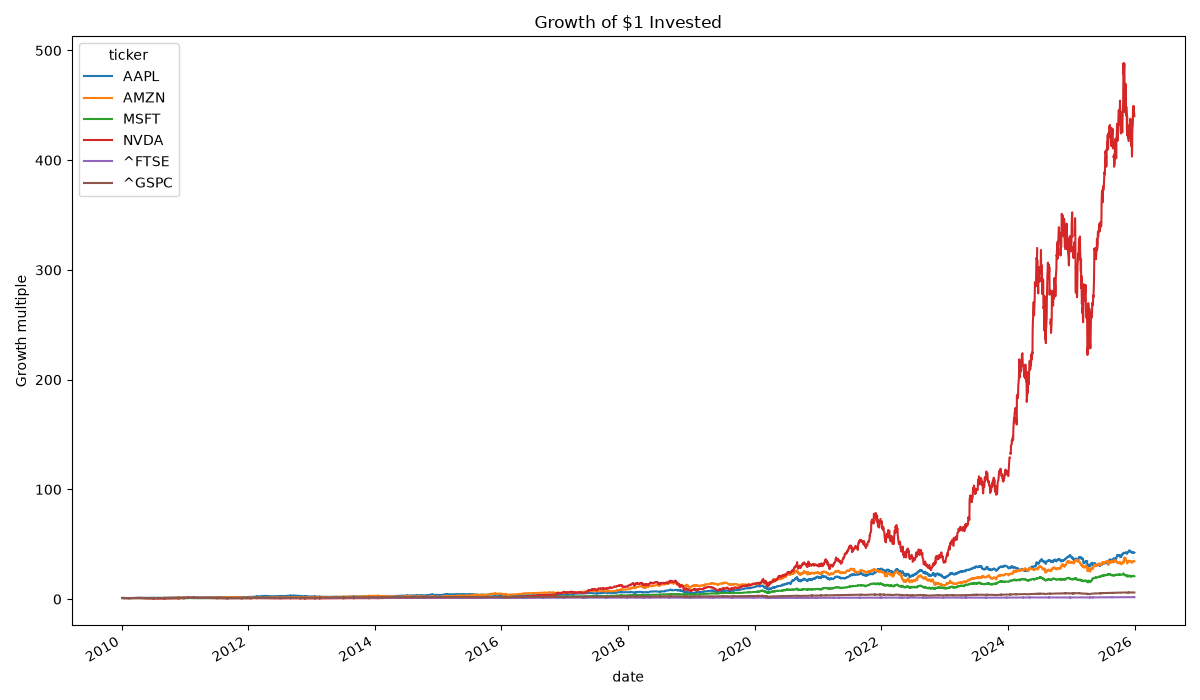
\includegraphics[width=0.95\textwidth]{figures/normalized_price_growth.png}
\caption{Normalised price growth from 2010 to 2025.}
\label{fig:growth}
\end{figure}

The chart shows that NVIDIA separated sharply from the other assets, especially in the later years of the dataset. This supports the total return results in Table \ref{tab:summary}. However, the chart also shows that NVIDIA's growth was not smooth. There were periods of sharp rises and large falls, which is consistent with its high volatility and large maximum drawdown.

Apple, Amazon, and Microsoft also grew strongly over the period. The S\&P 500 rose more steadily, while the FTSE 100 had the weakest long-term growth. This does not mean the FTSE 100 had no value as an investment, but in this selected dataset it did not produce the same level of growth as the US technology stocks.

\subsection{Daily Return Boxplot}

Figure \ref{fig:boxplot} shows the distribution of daily returns for each asset.

\begin{figure}[H]
\centering
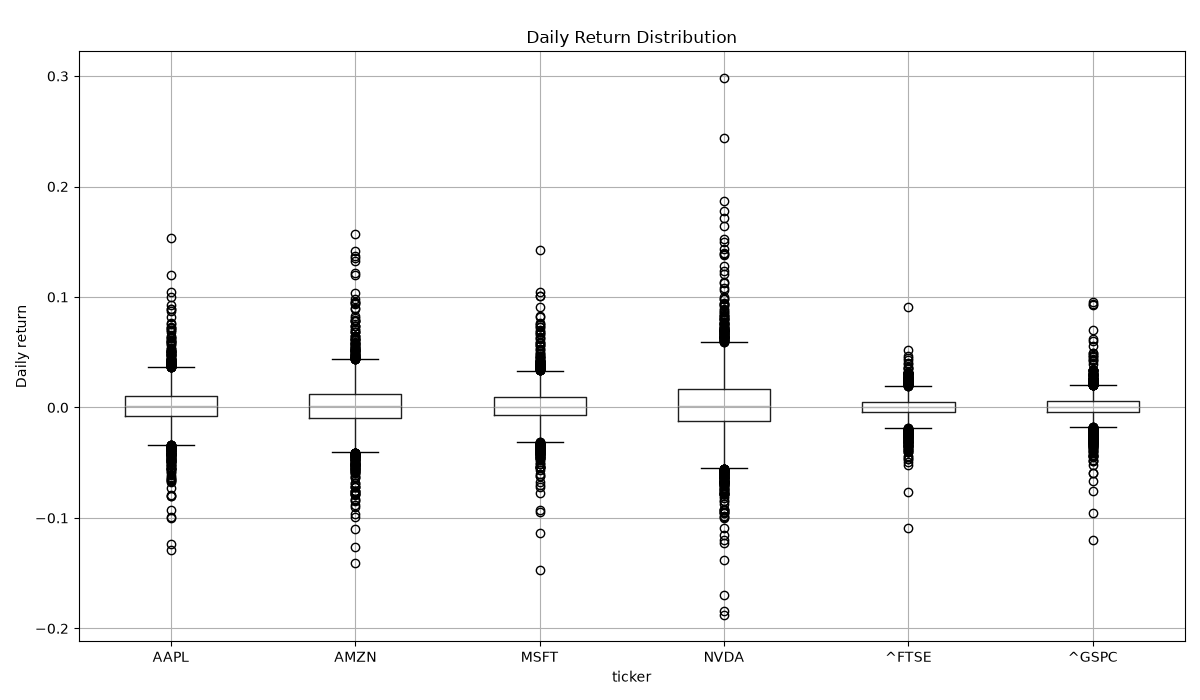
\includegraphics[width=0.95\textwidth]{figures/daily_return_boxplot.png}
\caption{Daily return distribution by asset.}
\label{fig:boxplot}
\end{figure}

This boxplot is one of the most important charts in the exploratory analysis because it shows the short-term risk behaviour of each asset. Each box summarises thousands of daily percentage returns.

The middle line inside each box is the median daily return. The median is the middle value when all daily returns are ordered from lowest to highest. In this chart, the medians are close to zero for every asset. This is normal for daily stock returns. Even assets that grew strongly over the long term usually have small daily movements, and many individual trading days are close to flat.

The bottom and top of each box represent the first quartile and third quartile. The first quartile is the point below which 25\% of daily returns fall. The third quartile is the point below which 75\% of daily returns fall. The height of the box is called the interquartile range. A taller box means the asset's typical daily returns were more spread out. A shorter box means the asset's daily returns were more stable.

NVIDIA has the widest box in the chart. Its middle 50\% of daily returns ranged approximately from -1.24\% to 1.63\%. This means that even on relatively normal trading days, NVIDIA tended to move more than the other assets. Amazon also had a relatively wide box, with its middle 50\% of daily returns ranging approximately from -0.91\% to 1.20\%. By contrast, the S\&P 500 and FTSE 100 had much narrower boxes, showing more stable daily movements.

The whiskers extend from each box to show the range of values that are not treated as outliers under the boxplot rule. Values beyond the whiskers are shown as individual dots. These dots represent unusually large positive or negative daily returns. They do not necessarily mean the data is wrong. In financial markets, outliers often represent major news events, earnings announcements, crashes, recoveries, or periods of extreme market stress.

NVIDIA has the most extreme outliers. Its best daily return was approximately 29.8\%, while its worst daily return was approximately -18.8\%. This is much more extreme than the broad market indices. The S\&P 500's best daily return was about 9.5\%, and its worst daily return was about -12.0\%. The FTSE 100 had a best daily return of about 9.1\% and a worst daily return of about -10.9\%.

The boxplot also helps explain why NVIDIA had the highest annualized volatility. Volatility is based on the spread of returns, and NVIDIA's returns are visibly more spread out than the others. Its wider box and longer outlier tails show that it experienced both larger normal daily movements and more extreme unusual movements.

The main conclusion from the boxplot is that high-growth stocks did not only grow more; they also moved around more from day to day. NVIDIA, Amazon, Apple, and Microsoft had larger daily return ranges than the S\&P 500 and FTSE 100. The indices were more stable because they represent diversified baskets of companies rather than a single company.

\subsection{Correlation Heatmap}

Figure \ref{fig:correlation} shows the correlation between the daily returns of each pair of assets.

\begin{figure}[H]
\centering
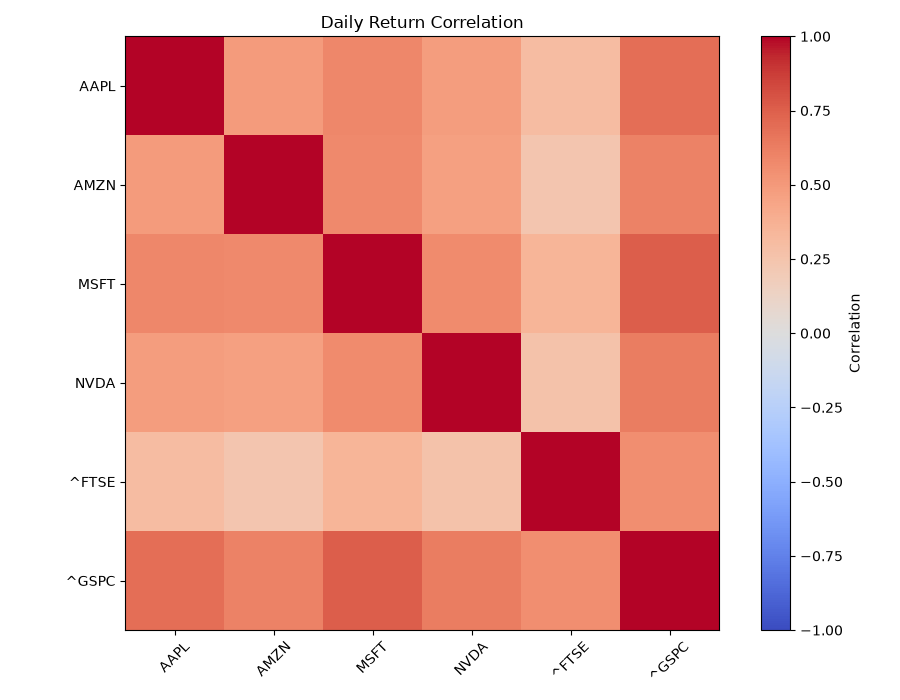
\includegraphics[width=0.85\textwidth]{figures/return_correlation_heatmap.png}
\caption{Daily return correlation heatmap.}
\label{fig:correlation}
\end{figure}

The strongest relationship was between Microsoft and the S\&P 500, with a correlation of approximately 0.75. This means Microsoft often moved in the same direction as the wider US stock market. Apple and the S\&P 500 also had a strong correlation of approximately 0.69.

The FTSE 100 had weaker correlations with the individual US technology stocks. This is expected because the FTSE 100 represents the UK market, while Apple, Microsoft, NVIDIA, and Amazon are US companies. The FTSE 100 still had a moderate correlation with the S\&P 500 of approximately 0.55, suggesting that global stock markets often move together, especially during broad market events.

\section{Discussion}

\subsection{Which Asset Grew the Most?}

NVIDIA grew the most over the study period. Its total return was approximately 43,906\%, far higher than Apple, Amazon, Microsoft, the S\&P 500, and the FTSE 100. This result reflects NVIDIA's rapid long-term growth, especially as demand for graphics processing units, data-centre computing, and artificial intelligence hardware increased.

However, this high return should not be interpreted in isolation. NVIDIA also had the highest volatility and the largest maximum drawdown. This means investors would have needed to tolerate large swings in value to earn the long-term return.

\subsection{Which Asset Was the Riskiest?}

NVIDIA was the riskiest asset based on annualized volatility. Its annualized volatility was approximately 45.7\%. Amazon was the second most volatile at approximately 32.8\%, followed by Apple at 28.2\% and Microsoft at 25.5\%.

The S\&P 500 and FTSE 100 were less volatile because they are indices rather than individual stocks. An index contains many companies, so poor performance in one company can be partly balanced by better performance elsewhere. This is the basic principle of diversification.

\subsection{Which Asset Had the Worst Drawdown?}

NVIDIA had the worst maximum drawdown, falling approximately 66.3\% from a previous peak at its worst point. Amazon also had a large maximum drawdown of about 56.1\%.

Maximum drawdown is important because it gives a more realistic view of investor experience. A final return can look excellent, but an investor still has to remain invested through difficult periods to receive it. A 66\% drawdown would be emotionally and financially challenging for many investors.

\subsection{Which Assets Moved Together?}

The strongest correlation was between Microsoft and the S\&P 500. This suggests that Microsoft behaved similarly to the wider US market during the study period. Apple, NVIDIA, and Amazon also had positive correlations with the S\&P 500.

All correlations in the table were positive, meaning the assets generally tended to move in the same direction rather than opposite directions. This matters for portfolio construction. If all assets are positively correlated, diversification can still reduce risk, but it may not protect the portfolio completely during broad market downturns.

\subsection{Was Higher Return Linked to Higher Risk?}

The analysis suggests that higher return was generally linked with higher risk. NVIDIA had the highest return and the highest volatility. Amazon and Apple also had high returns and higher volatility than the broad market indices.

However, the relationship was not perfect. Microsoft had a lower total return than Apple and Amazon, but it had a strong Sharpe ratio. This means Microsoft produced attractive return relative to the amount of volatility it experienced. For investors, this distinction matters because the best investment is not always the one with the highest raw return. Risk-adjusted return can provide a more balanced view.

\section{Limitations}

This analysis has several limitations.

First, the selected assets are limited. Four of the six assets are large US technology companies, so the results are strongly influenced by the performance of the technology sector. A broader study could include financial companies, healthcare companies, energy companies, bonds, commodities, and international markets.

Second, the project uses historical data. Past performance does not guarantee future performance. NVIDIA's historical growth was extremely strong, but that does not mean the same growth will continue.

Third, this analysis does not include dividends, transaction costs, taxes, inflation, or currency conversion effects. These factors can affect real investor returns.

Fourth, the Sharpe ratio uses a simplified assumption of a zero risk-free rate. A more advanced version would subtract the return available from a low-risk asset such as government bonds.

Finally, correlation is measured using daily returns across the full period. Correlations can change over time, especially during market crises.

\section{Conclusion}

This report analysed stock market risk and return using historical daily data from 2010 to 2025. The strongest long-term performer was NVIDIA, which produced a total return of approximately 43,906\%. However, NVIDIA was also the most volatile asset and had the largest maximum drawdown.

The daily return boxplot showed that most daily returns were close to zero, but individual technology stocks had wider distributions and more extreme outliers than the market indices. This means their daily performance was less stable. The S\&P 500 and FTSE 100 had narrower return distributions, reflecting the stabilising effect of diversification.

The correlation analysis showed that the US technology stocks were positively correlated with the S\&P 500, especially Microsoft. The FTSE 100 was less strongly correlated with the US technology stocks, although it still had a moderate relationship with the S\&P 500.

Overall, the analysis supports the idea that higher return often comes with higher risk. NVIDIA delivered exceptional growth, but investors had to accept high volatility and deep drawdowns. Microsoft provided an example of a stock with a strong balance between return and risk. These findings show why investors should consider volatility, drawdown, and correlation alongside total return when evaluating investments.

\section{Possible Future Work}

Future stages of this project could extend the analysis in several ways:

\begin{itemize}
    \item Calculate rolling volatility to see how risk changed over time.
    \item Analyse specific market crash periods, such as the COVID-19 crash.
    \item Build a portfolio simulator using a hypothetical investment amount, such as \pounds 10,000.
    \item Compare equal-weighted and risk-adjusted portfolios.
    \item Add dividend-adjusted returns.
    \item Build an interactive dashboard using Streamlit or Power BI.
    \item Test a simple machine learning model for next-day price direction, while evaluating it honestly.
\end{itemize}

\end{document}
